%!TEX root = ./main.tex
\documentclass[conference]{IEEEtran}
\IEEEoverridecommandlockouts
% The preceding line is only needed to identify funding in the first footnote. If that is unneeded, please comment it out.
\usepackage{cite}
\usepackage{amsmath,amssymb,amsfonts}
\usepackage{algorithmic}
\usepackage{graphicx}
\usepackage{textcomp}
\usepackage{xcolor}
\usepackage[utf8]{inputenc}
\usepackage{array}
\usepackage{gensymb}
\usepackage{mathtools}
\usepackage{units}
\usepackage{esvect}
\usepackage{multirow}
\usepackage{tikz}
\usepackage{subfig}
\usepackage{url}
\usepackage{listings}
\usepackage[ngerman]{babel}
\usepackage{enumerate}% http://ctan.org/pkg/enumerate

\newcommand{\code}{\texttt}
\renewcommand{\lstlistingname}{Quellcode}

\colorlet{punct}{red!60!black}
\definecolor{background}{HTML}{FFFFFF}
\definecolor{delim}{RGB}{20,105,176}
\colorlet{numb}{magenta!60!black}

\lstdefinelanguage{json}{
basicstyle=\normalfont\ttfamily,
numberstyle=\scriptsize,
stepnumber=1,
numbersep=8pt,
showstringspaces=false,
breaklines=true,
frame=lines,
backgroundcolor=\color{background},
literate=
*{0}{{{\color{numb}0}}}{1}
{1}{{{\color{numb}1}}}{1}
{2}{{{\color{numb}2}}}{1}
{3}{{{\color{numb}3}}}{1}
{4}{{{\color{numb}4}}}{1}
{5}{{{\color{numb}5}}}{1}
{6}{{{\color{numb}6}}}{1}
{7}{{{\color{numb}7}}}{1}
{8}{{{\color{numb}8}}}{1}
{9}{{{\color{numb}9}}}{1}
{:}{{{\color{punct}{:}}}}{1}
{,}{{{\color{punct}{,}}}}{1}
{\{}{{{\color{delim}{\{}}}}{1}
{\}}{{{\color{delim}{\}}}}}{1}
{[}{{{\color{delim}{[}}}}{1}
{]}{{{\color{delim}{]}}}}{1},
}


\lstdefinelanguage{epl}{
basicstyle=\normalfont\ttfamily,
numberstyle=\scriptsize,
stepnumber=1,
numbersep=8pt,
showstringspaces=false,
breaklines=true,
frame=lines,
backgroundcolor=\color{background}
}

\DeclarePairedDelimiter\ceil{\lceil}{\rceil}
\DeclarePairedDelimiter\floor{\lfloor}{\rfloor}

\def\BibTeX{{\rm B\kern-.05em{\sc i\kern-.025em b}\kern-.08em
    T\kern-.1667em\lower.7ex\hbox{E}\kern-.125emX}}
\begin{document}

%\title{TODO: globaleventprognosis}
%\title{Event Detection für Verhaltsmuster von Wikipedia-Nutzern}
%\title{Event Detection in Verhaltensmustern von Wikipedia-Nutzern}
%\title{Event Detection in Verhaltensmustern von Wikipedia-Artikeln}
\title{Event Detection in Wikipedia}


\author{\IEEEauthorblockN{Phillip Ginter}
\IEEEauthorblockA{\textit{Informatik (IN)} \\
\textit{Hochschule Furtwangen}\\
78120 Furtwangen, Deutschland \\
phillip.ginter@hs-furtwangen.de}
\and
\IEEEauthorblockN{Daniel Schönle}
\IEEEauthorblockA{\textit{Informatik (IN)} \\
\textit{Hochschule Furtwangen}\\
78120 Furtwangen, Deutschland \\
daniel.schoenle@hs-furtwangen.de}
}

\maketitle

% INPUT Content sections
%!TEX root = ./../main.tex
\begin{abstract}
Die freie Online-Enzyklopädie Wikipedia umfasst über 74 Millionen Artikel, die dauerhaft Änderungen unterzogen sind.
Auslöser für diese Änderungen können vielfältig sein. Ereignisse der realen Welt wie z.\,B. die Wahl des deutschen Bundeskanzlers
    führen zu einem starken kurzzeitigen Anstieg der Änderungen an dem entsprechenden Wikipedia-Artikel. Das Ziel dieser Arbeit
ist die Erkennung von Ereignissen der realen Welt, anhand von Änderungen an Wikipedia-Artikeln.
Für die Überwachung und Analyse der Änderung an Wikipedia-Artikeln wird eine Streaming-Data-Architektur entworfen und prototypisch umgesetzt.
    Die Modellierung von Mustern liefert dabei nicht die gewünschten Ergebnisse, weshalb der Einsatz eines Burst-Detection-Algorithmus vorgezogen wird.
TODO: Ziel erreicht, fehlt noch?
\end{abstract}

\begin{IEEEkeywords}
wikipedia, prognosis, global event
\end{IEEEkeywords}
%!TEX root = ./../main.tex
\section{Einleitung}
Wikipedia ist eine freie Online-Enzyklopädie, mit dem Ziel „eine frei lizenzierte und hochwertige Enzyklopädie zu schaffen und damit lexikalisches Wissen zu verbreiten“ \cite{wales.}. Sie umfasst 74 Millionen Artikel, die von eine Commuity von 137.571 Nutzer erstellt und geprüft wurden. Seit 2001 wurden die Artikel 877.073.914 mal editiert, dies entspricht etwa 4.000.000 Edit pro Monat. \cite{wikistat}.
TODO
Aufgrund des kollaborativen Erstellungsprozesses können \cite{wikipedia.}

TODO
Aufgabenstellung hier wiedergeben

\begin{itemize}
    \item Was ist Wikipedia?
    \item Wie viele Artikel, Edits, Autoren hat Wikipedia?\footnote{https://en.wikipedia.org/wiki/Wikipedia:Statistics}
    \item Ein Edit bzw. Update in Wikipedia wird durch ein neues Ereignis der realen Welt ausgelöst. Das kann eine Wahl,
    ein Unfall, politische Konflikte oder eine Sportveranstaltung sein \cite{10.1007978-3-642-36973-5_22}.
    \item Aufgabenstellung
    \begin{itemize}
        \item Für eine Entität (z. B. eine Person des öffentlichen Lebens) aus der Gesamtheite der Wikipedia-Edit-Events in "Echtzeit"
        Events der realen Welt ableiten.
        \item Wir betrachten nur die Metadaten (Zeitstempel, Autor, ...) und nicht den Inhalt der Änderung Änderung (z. B. textuelle Änderung).
        \item ...
    \end{itemize}
    \item Wie sieht so ein Burst of Wikipedia-Edits aus \ref{fig:donald_rumsfelds_resignation_burst}?
\end{itemize}


\begin{figure}[h]
    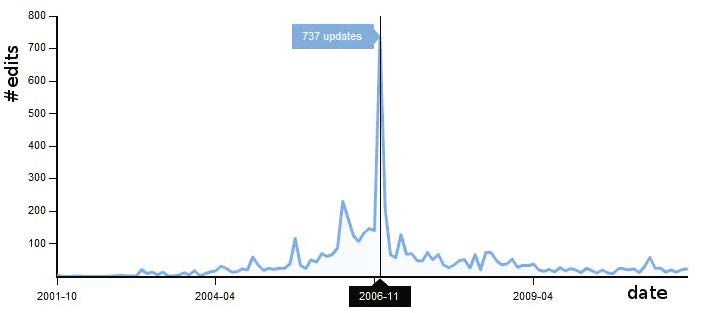
\includegraphics[width=.5\textwidth]{images/Extracting_EventRelated_Information_from_Article.jpg}
    \caption{Donald Rumsfeld’s Rücktritt führte zu einem Burst an Autoren, die einen Wikipedia-Edit vornahmen \cite{10.1007978-3-642-36973-5_22}.}
    \label{fig:donald_rumsfelds_resignation_burst}
\end{figure}
\section{Verwandte Arbeiten}
\subsection{Burst Detection}
Generell

Kleinberg’s burst detection algorithm

Online Burst Detection Over High Speed Short Text Streams

Event Detection with Burst Information Networks

Realtime
Die Realtime-Burst Detection über mehrere Fenstergrößen ist für die Analyse von Datenströmen hilfreich. Die üblichen Burst-Detektionsverfahren sind für die Echtzeiterkennung nicht effektiv. Die Realtime-Burst Detection benötigt eine neue Burst-Erkennungsmethode, die die Berechnung reduziert, indem redundante Datenaktualisierungen vermieden werden. Dabei wird ein Ereignis bei seinem Auftreten daraufhin analysiert inwiefern die Ankunftshäufigkeitund eim Vergleich zur vorherigen Perioden ansteigt.

Efficient Elastic Burst Detection in Data Streams 

\cite{10.1007978-3-642-36973-5_22}
%!TEX root = ./../main.tex
\section{Streaming-Data}

Das Ziel unserer Aufgabenstellung ist die Verarbeitung von Streaming-Daten in Echtzeit. Die Streaming-Data-Architektur
von Psaltis \cite{psaltis2017streaming} ist für diese Art von Problem konzipiert und bildet die Grundlage für
unsere Architektur. Nach der kurzen Vorstellung der Streaming-Data-Architektur von Psaltis, zeigen wir unsere eigene konkrete
Umsetzung und vergleichen eingesetzten Technologien mit Alternativen.

\subsection{Streaming-Data-Architektur nach Psaltis}

In Abbildung \ref{fig:streaming_data_architecture-psaltis} sind die Komponenten der Streaming-Data-Architektur, wie Psaltis \cite{psaltis2017streaming}
sie entwickelt hat, abgebildet. Der Collection-Tier ist der Einstiegspunkt, der Daten in das System bringt. Unabhängig von dem verwendeten
Protokoll, werden die Daten mithilfe eines dieser Patterns übertragen \cite{psaltis2017streaming}:
\begin{itemize}
    \item Request/response pattern
    \item Publish/subscribe pattern
    \item One-way pattern
    \item Request/acknowledge pattern
    \item Stream pattern
\end{itemize}

Bei der Datenquelle kann es sich sowohl um von Hardware und auch von Software generierte Events handeln. Beispiele hierfür sind
Temperatur, Lautstärke oder auch Browser-Clicks.


\begin{figure*}
    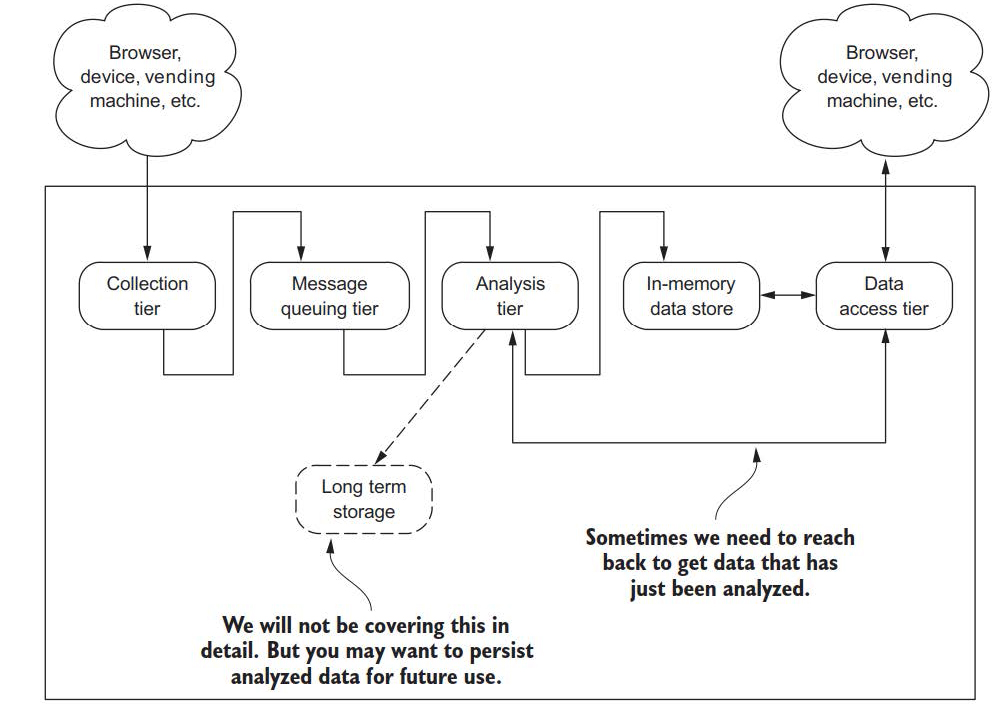
\includegraphics[width=\textwidth]{images/streaming_data_architecture-psaltis.jpg}
    \caption{Streaming-Data-Architektur \cite{psaltis2017streaming}}
    \label{fig:streaming_data_architecture-psaltis}
\end{figure*}


Um die Daten vom Collection-Tier auf den Rest der Pipeline zu verteilen wird ein Messaging Queuing Tier implementiert.
Das Message-Queuing-Model ist ein Modell zur Interprozesskommunikation. Anwendungen schicken
Nachrichten an eine Nachrichtenschlange, von der andere Anwendungen diese abholen können \cite{gray2003interprocess}.
Dadurch werden die eingesetzten Systeme voneinander entkoppelt und die Kommunikation findet nicht durch direkte Aufrufe,
sondern über die Queue statt \cite{psaltis2017streaming}. Im vorliegenden Fall wird der Collection-Tier vom Rest der Pipeline entkoppelt.

Im Analysis-Tier werden auf die Streams des Message-Queuing-Tiers kontinuierlich Queries angewandt um Muster in den Daten zu erkennen.
Hier können Event-Stream-Processing-Systeme (ESP) wie z.\,B. Apache Flink, Apache Spark oder Apache Storm oder
auch Complex-Event-Processing-Systeme (CEP) wie z.\,B. Esper oder Apache Samza eingesetzt werden \cite{psaltis2017streaming}.
In ESP wird die Verarbeitungslogik imperativ umgesetzt, wohingegen CEP einen deklarativen Ansatz verfolgt.
Die Event-Processing-Languages (EPL) sind Sprachen, die über Sequenz-, Konjunktions-, Disjunktions- und Negationsoperatoren
verfügen und für CEP entwickelt wurden \cite{hedtstck2017complex}. Als Basis der Operatoren werden Windows eingesetzt.
Ist die Analyse vorbei und die Ergebnisse stehen fest, können die Ergebnisse verworfen werden, zurück in die Streaming-Plattform gespeichert werden,
für eine Echtzeitnutzung oder die Stapelverarbeitung gespeichert werden \cite{psaltis2017streaming}. Wie der Abbildung \ref{fig:streaming_data_architecture-psaltis}
zu entnehmen ist, schlägt Psaltis hierfür eine In-Memory-Datenbank (IMDB), einen Data-Access-Tier und ein Long-Term-Storage vor.
Je nach Anwendungsfall ist das eine System dem anderen überlegen.

\subsection{Unsere Streaming-Data-Architektur}
In diesem Kapitel geht es um die Frage, welche Technologie wir in dem jeweiligen Tier einsetzen und wieso wir uns dafür entschieden haben.
Technische Details, die die Implementierung betreffen, erläutern wir im nächsten Kapitel.
%TODO: Quellen zu den einzelnen Punkten/Systemen
\begin{itemize}
    \item \textit{Collection-Tier.} Als Datenquelle nutzen wir die frei zugänglichen Daten von Wikipedia. Konkret handelt es sich um die Recent-Changes,
    also die aktuellen Änderungen an Wikipedia-Einträgen. Details hierzu sind im nächsten Kapitel beschrieben. Wir entschieden uns für Wikipedia als
    Datenquelle, weil es eine offene Plattform ist, die einen freien Zugang zu allen Daten gibt.

    \item \textit{Messaging-Queuing-Tier.} Wir nutzen Kafka als Messaging-System, weil es skalierbar ist, einen hohen Datendurchsatz ermöglicht,
    Real-Time-Messaging unterstützt, eine einfache Client-Anbindung ermöglicht und Events standardmäßig persistiert \cite{chellappan2018practical}. Der letzte Punkt ist
    besonders relevant, da für die Entwicklung der Regeln eine statische Datenmenge einfacher zu handhaben ist.

    \item \textit{Analysis-Tier.} Die Analyse der Wikipedia-Edit-Events sollte deklarativ erfolgen. Dadurch erhofften wir uns
    in kurzer Zeit eine Vielzahl an Regeln zu testen und so ein gutes Verständnis für die Daten zu erhalten. Aufgrund dieser Vorgabe
    entschieden wir uns für Esper. Es bietet eine CEP-Implementierung, die nach einem regelbasierten Ansatz -- somit deklarativ -- arbeitet.
    Ein weiterer Punkt, der für Esper sprach, war zum einen die Esper Processing Language und die Implementierung der Anwendung in Java.

    \item \textit{In-Memory-Data-Store, Long-Term-Storage und Data-Access-Tier.} Für diese drei Komponenten haben wir selbst keine Implementierung vorgesehen.
    Im Ausblick geben wir hierzu Ideen zu möglichen Weiterentwicklungen.
\end{itemize}
%!TEX root = ./../main.tex
\section{Prototyp}
Zur Lösung der Aufgabenstellung haben wir einen lauffähigen Prototypen entwickelt, der die Machbarkeit demonstriert.
Dafür haben wir die im vorhergehenden Kapitel genannten Technologien eingesetzt. Die Details zu den jeweils entstandenen
Anwendungen stellen wir in diesem Kapitel vor.

\begin{figure*}
    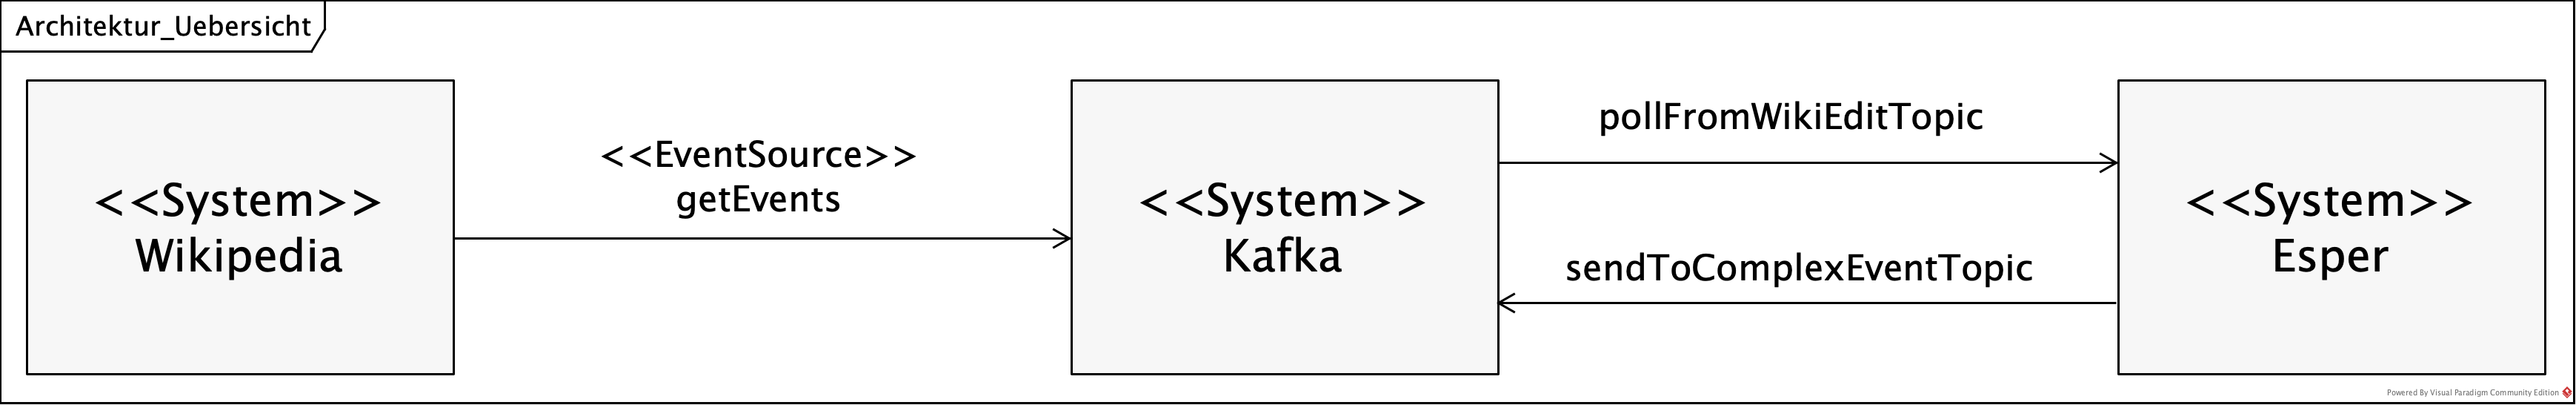
\includegraphics[width=\textwidth]{images/Architektur_Uebersicht.png}
    \caption{Architekturübersicht}
    \label{fig:architektur_uebersicht}
\end{figure*}

Abbildung \ref{fig:architektur_uebersicht} zeigt die Teilsysteme und deren Interaktion untereinander.

% Abbildung \ref{fig:architektur_uebersicht} zeigt bisher nur eine sehr rudimentäre Übersicht und soll als Grundlage dienen.
% Die Verbindung zwischen Esper und Kafka muss noch genauer werden: Protokoll, senden von komplexen Events in neue Kafka-Topics.

\subsection{Collection Tier: Wikipedia}
Wie zuvor beschrieben, stützt sich unser System auf Daten von Wikipedia. Wir nutzen den RecentChanges-Stream, der
Events zu neu erstellten, aktualisierten und gelöschten Wikipedia-Seiten enthält\footnote{https://www.mediawiki.org/wiki/Manual:RCFeed}.
Der Quellcode \ref{WikipediaRecentChangeJSON} zeigt einen Ausschnitt eines solchen Events.
Es sind nur die Attribut abgebildet, die in einem der nachfolgenden Teilsysteme relevant sind.

\begin{lstlisting}[label=WikipediaRecentChangeJSON,caption=Wikipedia RecentChange-Event,language=json,firstnumber=1,captionpos=b]
{
    "bot": false,
    "comment": "/* Politischer Werdegang */",
    "id": 269108829,
    "meta": {
        "uri": "https://de.wikipedia.org/wiki/Ingeborg_H%C3%A4ckel",
        "partition": 0,
        "offset": 1329388977
    },
    "timestamp": 1547910734,
    "title": "Ingeborg H\"ackel",
    "user": "Eszet2000",
    "wiki": "dewiki"
}
\end{lstlisting}

Die beiden Parameter \code{offset} und \code{uri}, innerhalb des \code{meta}-Objektes, stammen aus einem Kafka-System
und dienen der Wiederaufnahme eines abgebrochenen Streams. Wikipedia setzt intern Apache Kafka als Messaging-System ein.
Nach außen nutzt Wikipedia EventStreams. Das ist ein Webservice der kontinuierliche Datenströme mit strukturierten Daten
über HTTP sendet\footnote{https://wikitech.wikimedia.org/wiki/EventStreams}. Die Basis-Technologie dessen, ist
das Server-Sent Event (SSE) Protokoll. Der RecentChanges-Stream ist ein solcher Stream und kann über eine Client-Bibliothek
konsumiert werden.

Wie im vorherigen Kapitel beschrieben, werden Daten vom Collection Tier mithilfe eines der aufgelisteten Pattern übertragen.
SSE funktioniert nach dem One-way pattern, indem eine HTTP-Verbindung aufgemacht wird um Nachrichten zu empfangen \cite{EventSource_SSE}.

\subsection{Implementierungsdetails zum Messaging Queuing Tier: Kafka}
Im Messaging Queuing Tier setzen wir Apache Kafka in der Version 2.1 ein, um die im Collection Tier beschriebenen Wikipedia-Events
in unser eigenes Messaging-System zu überführen. Hierfür haben wir eine Java-Anwendung entwickelt, in der die folgenden
Schritte nacheinander ausgeführt werden:
\begin{enumerate}
    \item \textit{Kafka Initialisierung.} Den Host des Bootstrap-Servers setzen um eine Verbindung zu erzeugen.
    Als Key- und Value-Serialisierer setzen wir
    jeweils den \code{StringSerializer} von Kafka ein. Das heißt, die Events werden als JSON-String in das Topic \code{wikiEdit}
    eingespeist. Zum Senden von Events erzeugen wir ein Producer-Objekt mit dem passenden Typ \code{Producer<String, String>}.
    An dieser Stelle war die Überlegung, anstelle eines String-Serialisierers für den Wert des Producers,
    einen eigenen Serialisierer für die WikipediaEditEvent-Klasse einzusetzen. Wir entschieden uns aber für den
    String-Serialisierer, da Wikipedia die Events auch als JSON-String überträgt und wir in Kafka selbst
    keine weiteren Operationen an den Daten vornehmen. Eine mögliche Operation könnte ein Filter sein.
    Aber das einzige Ziel von Kafka soll die Persistierung und Weitergabe von Daten sein und dafür ist keine Serialisierung in
    einem bestimmten Typen notwendig. Außerdem verschiebt es Komplexität aus der Kafka-Anwendung
    in die Consumer-Anwendungen.
    \item \textit{Erzeugung eines EventHandlers.} Für das Empfangen von EventSource-Nachrichten nutzen wir die Java-Bibliothek
    \textit{okhttp-eventsource}\footnote{https://github.com/launchdarkly/okhttp-eventsource}. Zur Verarbeitung der Events
    \code{onOpen}, \code{onClose}, \code{onMessage}, \code{onComment} und \code{onError} muss das Interface \code{EventHandler} von
    \textit{okhttp-eventsource} implementiert werden.
    \item \textit{Erzeugung und Starten einer EventSource.} Mit der Stream-URI der Wikipedia-EventSource (für die RecentChanges ist das: https://stream.wikimedia.org/v2/stream/recentchange)
    und des implementierten EventHandler-Interfaces
    kann ein \code{EventSource}-Objekt erzeugt werden. Das Objekt dient dem Starten und Beenden eines EventSource-Streams.
    Die Daten werden dann, wie zuvor beschrieben, durch das SSE-Protokoll von Wikipedia an die Anwendung gesendet.
    \item \textit{Beim Eintreffen eines Events: Senden einer Nachricht in ein Kafka-Topic.} Tritt ein Wikipedia-Event auf,
    wird die \code{onMessage}-Methode des implementierten EventHandlers-Interface aufgerufen. Der zweite Parameter enthält die Daten
    des aufgetretenen Events. Der Zugriff auf die als JSON-String codierte Nachricht erfolgt über die \code{getDate()}-Methode.
    Diese Daten sendet die Anwendung, über den zuvor erzeugten Producer, ohne eine weitere
    Verarbeitung in das Kafka-Topic \code{wikiEdit}.
\end{enumerate}

Die Konfiguration von Kafka ist sehr einfach gehalten, da es sich hierbei nur um einen Prototypen handelt.
Deswegen haben wir das eine Topic \code{wikiEdit}. Die Anwendung läuft nur auf einem Server, weshalb wir auch nur
eine Partition einsetzen und keine Replikation haben.

\subsection{Implementierungsdetails zum Analysis Tier: Esper}
In unserer Esper-Anwendung, die Teil des Analysis Tier ist, nutzen wir Esper in Version 7.1 als Complex Event Processing-Werkzeug. Zur Verarbeitung
der Wikipedia-Events implementieren wir die folgenden Schritte:

Genaueres zu den erzeugten Expressions im nächsten Kapitel.

Einsatz von GSON

\begin{enumerate}
    \item \textit{Esper Initialisierung.} Die Initialisierung von Esper besteht
    \item \textit{Expression erzeugen.}
    \item \textit{\code{UpdateListener} implementieren.}
    \item \textit{Kafka initialisieren.}
    \item \textit{Kafka Consumer erzeugen und in Endlosschleife Events pollen.}
    \item \textit{Empfangene Events auswerten.}
\end{enumerate}


\subsection{BurstDetection-Implementierung}
\section{Anwendungsfälle}
\subsection{Erkennung globaler Events}
Die Erkennung global relevanter Events wurde bereits in Kapitel \ref{sec:Einleitung} beschreiben.\\

Der Fokus bei der Umsetzung liegt dabei auf der Verarbeitung der Events in Echtzeit, dem Erkennen von Ereignismustern im Wikipedia-Edit-Eventsstrom und dem generieren von komplexen Events. Eine komplexe Datenanalyse ist nicht vorgesehen, statt dessen wird durch eine einfache Mustererkennung genutzt. Dabei werden Events innerhalb von Zeitfenstern aggregiert und in Beziehung zueinander gesetzt um Rückschlüsse auf 'Global Events' zu ziehen.\\

Die Zielsetzung, den Fokus auf das Erkennen von Ereignismustern in Wikipedia-Edit-Eventsstrom zu setzen und dabei auf komplexe Datenanalyse zu verzichten, schränkt die Anzahl erkannter 'Global Events' ein.\\

In der Realtime-Analyse kann ein Hinzuziehen externer Informationen nicht erfolgen. Deswegen sind Abfragen externer Quellen, eine Textanalyse der Änderungen auf die in den Edits verweisen wird, eine Verortung der Seite in der Wikipedia-Artikel-Hierarchie und das Parsen externer Web-Seiten zum Zweck der weiteren Informationsgewinnung nicht möglich. 

% Einfache Muster können in Echtzeit erkannt werden. Bei erfolgreicher Erkennung dieser Muster werden komplexe Events erzeugt. Dadurch erhöht sich die Informationsdichte im Stream und vergrößert die Granularität, verringt die Frequenz. Aufwändigeren Analysen werden daher an komplexe Events gebunden.


\subsection{Entworfene Anwendungsfälle}
Die Mustererkennung im Wikipedia-Edit-Stream kann für weitere Analysen verwendet werden. Exemplarisch wurden weitere Anwendungsfälle entwickelt, die sich im Umfeld der Wikipedia-Nutzer umsetzen lassen. Die vorgestellten Use Cases leiten sich aus Problemen kollaborativer Texterstellung und dem Nutzer verhalten ab.

\begin{itemize}
    \item Edit-Wars Detection\\ Bei Edit-Wars stimmen die Vorstellungen über den Inhalt des Artikels der Autoren nicht überein. Die Folge sind wiederholtes gegenseitiges Revidieren der Änderungen, häufig in hoher Frequenz.\cite{wikipediaprob.}\\ Daraus entstehen folgende Use Cases: Erkennen von aktiven Edit-Wars. Erkennen von Situationen die zu Edit-Wars führen. Identifizieren von Nutzern die im indirekten Zusammenhang mit Edit-Wars stehen.
    \item Fraud Detection\\Unter Vandalismus wird im Kontext der Wikipedia die Änderung von Textinhalten oder Bildern durch Benutzer mittels Einstellung offensichtlich unsinniger oder beleidigender, diffamierender, vulgärer oder obszöner Inhalte verstanden. Vandalismus wird typischerweise durch unangemeldete Benutzer verübt.\cite{wikipediaprob.} \\Use Cases: Ab wann gilt eine Änderung als Vandalismus? Gibt es Muster, die sich vor einem Vandalismus ereignen? 
    \item Nutzerkreise\\Im Zentrum stehen Nutzer die untereinander in Verbindung stehen.\\Use Cases: Gibt es Nutzergruppen die ähnliche thematische Expertise aufweisen? Bilden sich auch Metagruppen mit noch unbekannten Gemeinsamkeiten?
    \item Machtprozesse\\Wie in allen Organisationen entstehen auch in der Wikipedia Machtstrukturen.\\Use Cases:Bildet sich die Organisationshierarchie in den Edits ab? Lässt sich eine Tendenz zur Abschottung durch Selbstergänzung der Experten erkennen?\cite{wikipedia.}
    \item Request Prediction\\Die Menge der Nutzer-Anfragen an die Wikipedia-Serverinfrastruktur variiert vermutlich.\\Use Cases: Welche Muster lassen sich in der Nutzerlast erkennen? Ist das Interesse an bestimmten Artikel zu bestimmten Tageszeiten auffällig? Lässt sich die Nutzerlast vorhersagen?
    %\item Semantic-Clustering\\ \\Use Cases
\end{itemize}

%!TEX root = ./../main.tex
\section{Ergebnisse}
Die Anzahl und Verteilung der Änderungen an Wikipedia-Seiten sind zu verschieden, um daraus ein allgemeingültiges Muster für relevante Ereignisse abzuleiten.
Da ein relevantes Ereignis auch nicht auf jeder Wikipedia-Seite den selben Gesetzmäßigkeiten folgt, spielt die Betrachtung der vergangenen Events eine große Rolle.
Erst dadurch kann mithilfe eines Burst-Detection-Algorithmus ein relevantes Ereignis für einzelne Wikipedia-Seiten ermittelt werden.

Der Einsatz von Esper im Analysis-Tier, war für die erste Lösung die richtige Wahl. Wie sich jedoch gezeigt hat, konnten wir damit
nicht die gewünschten Ergebnisse erzielen. Die zweite Lösung war jedoch in Esper nicht in vollem Umfang umsetzbar.
Das Ziel, die Analyse von relevanten Ereignissen in Echtzeit, mussten wir auf die Betrachtung der 100 neuesten Events beschränken.
Denn Esper ermöglicht keinen Zugriff auf vergangene Events, wie es beispielsweise in Apache Flink, FlinkCEP mit Stateful Computation möglich ist\cite{Friedman:2016:IAF:3126171}.

\section{Ausblick}
Die Lösung 2 aus Kapitel \ref{section:prototyp} wurde nur auf deutschsprachige Wikipedia-Artikel und einen Zeitraum von 2 Tagen, in denen Wikipedia-Events gesammelt wurden, angewandt.
Das hatte den Vorteil, dass die Menge an Events und auch die zu erwartenden Ergebnisse überschaubar blieben und eine Validierung praktikabler machte.
Es bleibt somit offen, die Anwendbarkeit auf einen größeren Zeitraum und eine größere Menge an Events auszuweiten und die Testresultate zu validieren.

Des Weiteren können auf Basis der gewonnen Erkenntnisse im Analysis-Tier -- die Ebenen der Burst-Detection -- weitere Analysen durchgeführt werden.
Eine Möglichkeit ist es, für jede URI die Ebenen wieder zurück in ein Kafka-Topic zu senden. Dadurch können andere Analysis-Tier-Anwendungen diese zur Analyse einsetzen.
Zum anderen könnten die Ebenen über den Data-Access-Tier von außen aufrufbar gemacht werden. Ein konkretes Szenario hierfür ist eine Webseite
die für einzelne Wikipedia-Webseiten -- auf Basis der Ebenen -- eine Timeline mit den relevantesten Ereignissen darstellen kann.

\section{Beiträge der Autoren}
 Phillip Ginter und Daniel Schönle haben gleichermaßen zu dieser Arbeit beigetragen und sind Erstautoren.

% Quellenverzeichnis
\bibliographystyle{IEEEtran}
\bibliography{bibtex}

\end{document}
